\chapter{Vizualizace dostupnosti}

V~této kapitole řešíme problémy s~vizualizací ze sekce~\ref{problemyKReseni-vizualizace}. Abychom uživatelům usnadnili orientaci ve výsledcích a~umožnili jim snadné vyhledávání nejdostupnějších míst, vizualizujeme dostupnost na mapě. Vizualizace dělíme do dvou druhů, statické a~interaktivní.

\section{Výpočet dostupnosti pro body v~rastru} \label{optim-body}

Vizualizace dostupnosti na zastávkách je poměrně snadná. Problém nastane, chceme-li vizualizovat místa. Všech míst může být totiž nekonečně mnoho.

Potřebujeme tedy zvolit nějaké rozlišení, pro které budeme místa vizualizovat. Místa v~daném rozlišení rozmísťujeme pravidelně do mřížky. Takto uspořádaná místa nazveme rastrem.

Již pro rozlišení 100~x~100, tedy 10 000 míst trvá vyhodnocení dostupnosti v~místech řádově desítky sekund. Tento čas částečně zkrátíme využitím optimalizace popsané v~sekci~\ref{optim-sousedi}. Pro praktické použití je však tento výpočet příliš pomalý.

Nejnáročnější část výpočtu je hledání sousedních zastávek konkrétního bodu, které potřebujeme pro vyhodnocení dostupnosti. 

Při pevně daném rozlišení se však tyto body, ani jejich sousední zastávky nemění. Toho můžeme využít tak, že si sousední zastávky bodů vyhledáme předem. Dosáhneme tak výrazného zrychlení a~dostupnost pro stejných 10 000 bodů jsme schopni vypočítat za méně než jednu sekundu.

\section{Statické vizualizace}

Statické vizualizace můžeme využít pro zobrazení výsledků během vývoje aplikace. V~porovnání s~interaktivními vizualizacemi je jejich implementace poměrně snadná. Nejsou však příliš vhodné pro uživatele, neboť neumožňují snadné vyhledání nejdostupnějších míst.

\subsubsection{Implementace}

K~implementaci statických vizualizací jsme využili jazyk Python, neboť zpřístupňuje knihovny, které velice usnadňují práci s~daty a~jejich následnou vizualizaci.

Konkrétně jsme využili následující knihovny.

\begin{itemize}
    \item Pandas --- pro čtení dat ve formátu CSV.
    \item Shapely --- pro reprezentaci bodu pomocí souřadnic. 
    \item GeoPandas --- pro práci s~body.
    \item Contextily --- pro přidání podkladové mapy.
    \item Matplotlib --- pro vykreslení vizualizace.
\end{itemize}

\subsubsection{Vizualizace zastávek}

Dostupnost na zastávkách vizualizujeme pomocí barevných bodů, viz obrázek~\ref{fig:gtfs-mostAccessibleStop}. Pro souřadnice každé zastávky vykreslíme do mapy bod. Barva bodu je závislá na dostupnosti vypočtené pro zastávku pomocí algoritmu RAPTOR.

% prilis vysoky obrazek => je pak uzsi a hure citelny?
\begin{figure}[ht]
    \centering
    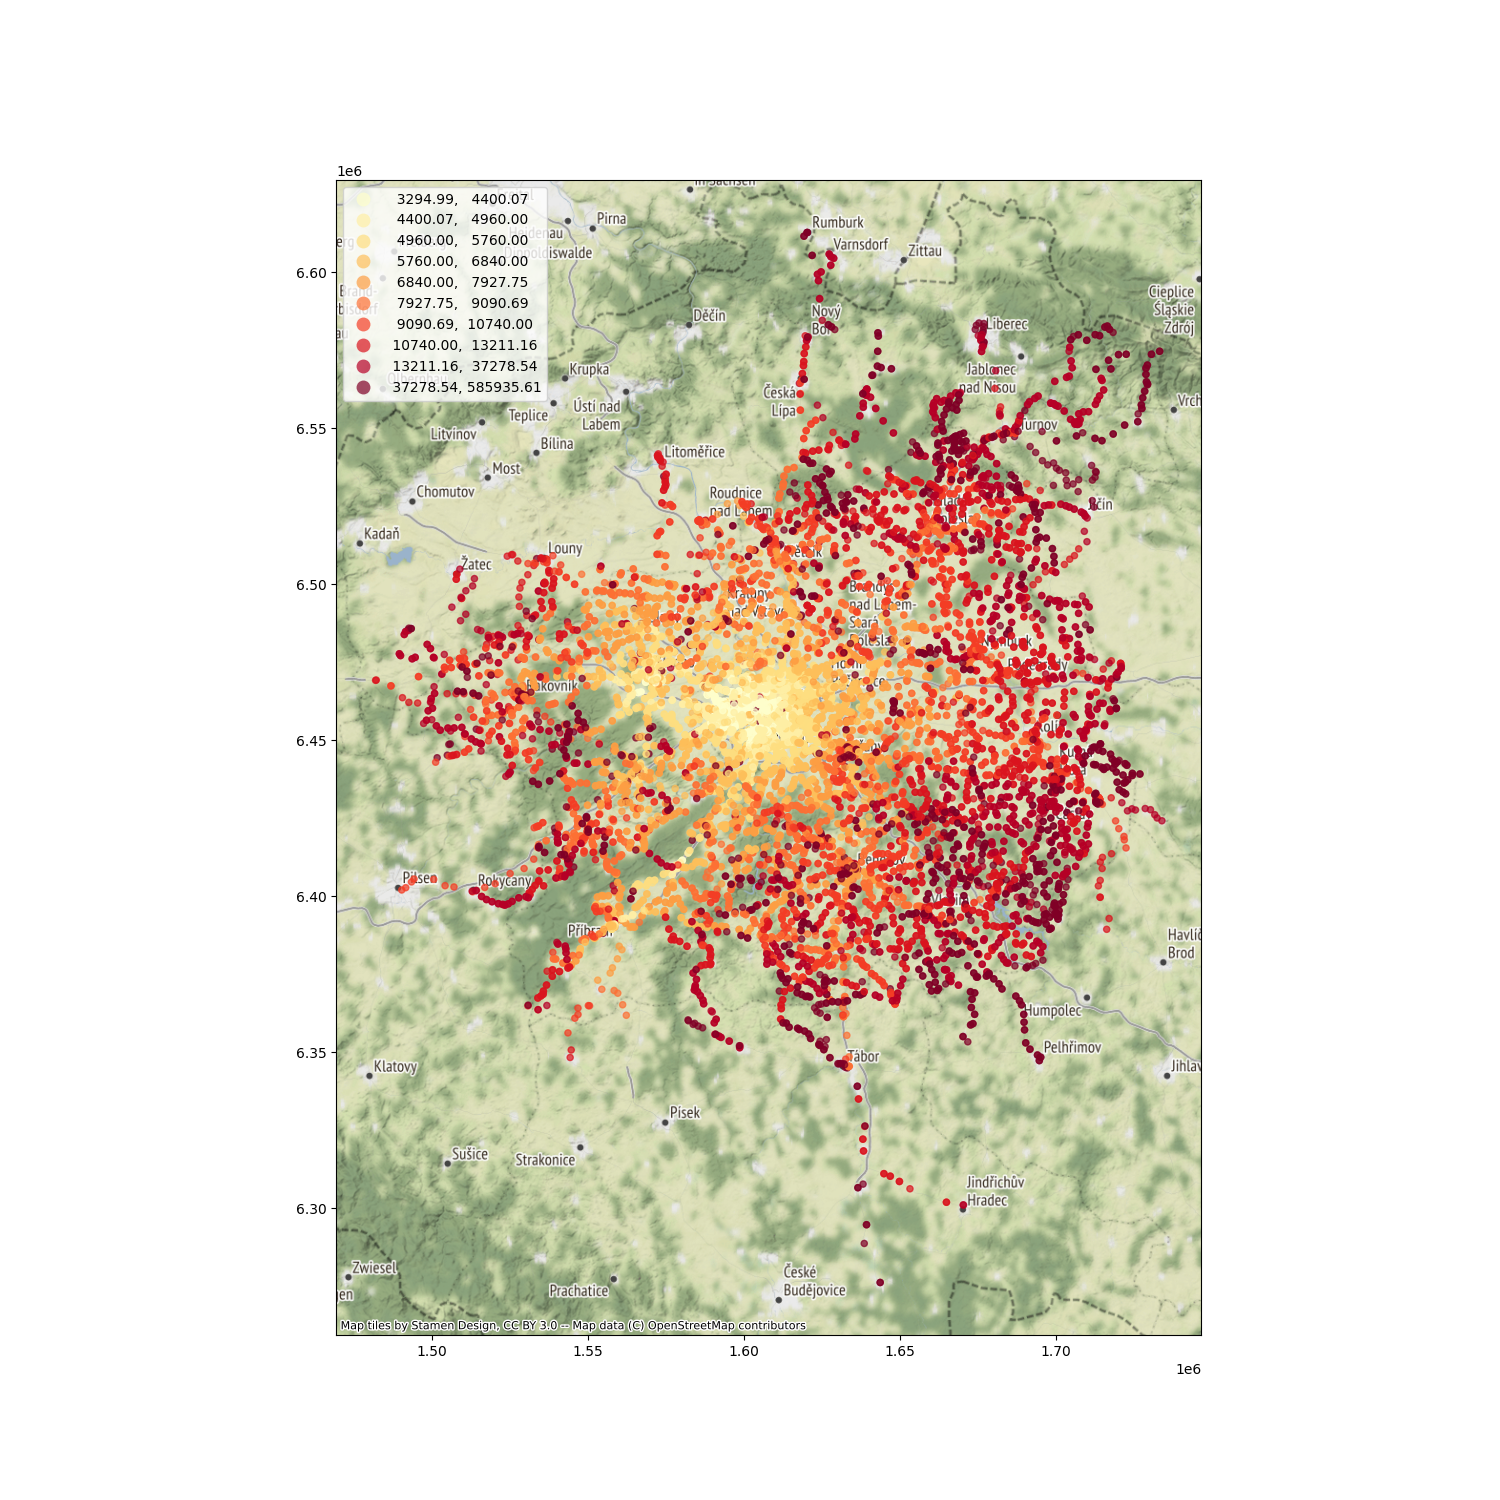
\includegraphics[width=\textwidth]{../img/staticStopsVisualization.png}
    \caption{Vizualizace dostupnosti na zastávkách z~Malostranského náměstí, Kladna a~Příbrami. Hodnoty v~legendě vyjadřují dostupnost v~sekundách.}
    \label{fig:gtfs-mostAccessibleStop}
\end{figure}

\subsubsection{Vizualizace míst}

Nejprve potřebujeme vybrat místa, která budeme vizualizovat. Místa budeme volit v~rastru. Tuto metodu jsme popsali i~s~optimalizací v~sekci~\ref{optim-body}.

Pro ohodnocení míst použijeme metodu popsanou v~sekci~\ref{zobecneni-ciloveZastavkyNaMista}.

Samotná vizualizace probíhá stejně jako vizualizace zastávek, viz obrázek~\ref{fig:gtfs-mostAccessiblePlace}.

\begin{figure}[ht]
    \centering
    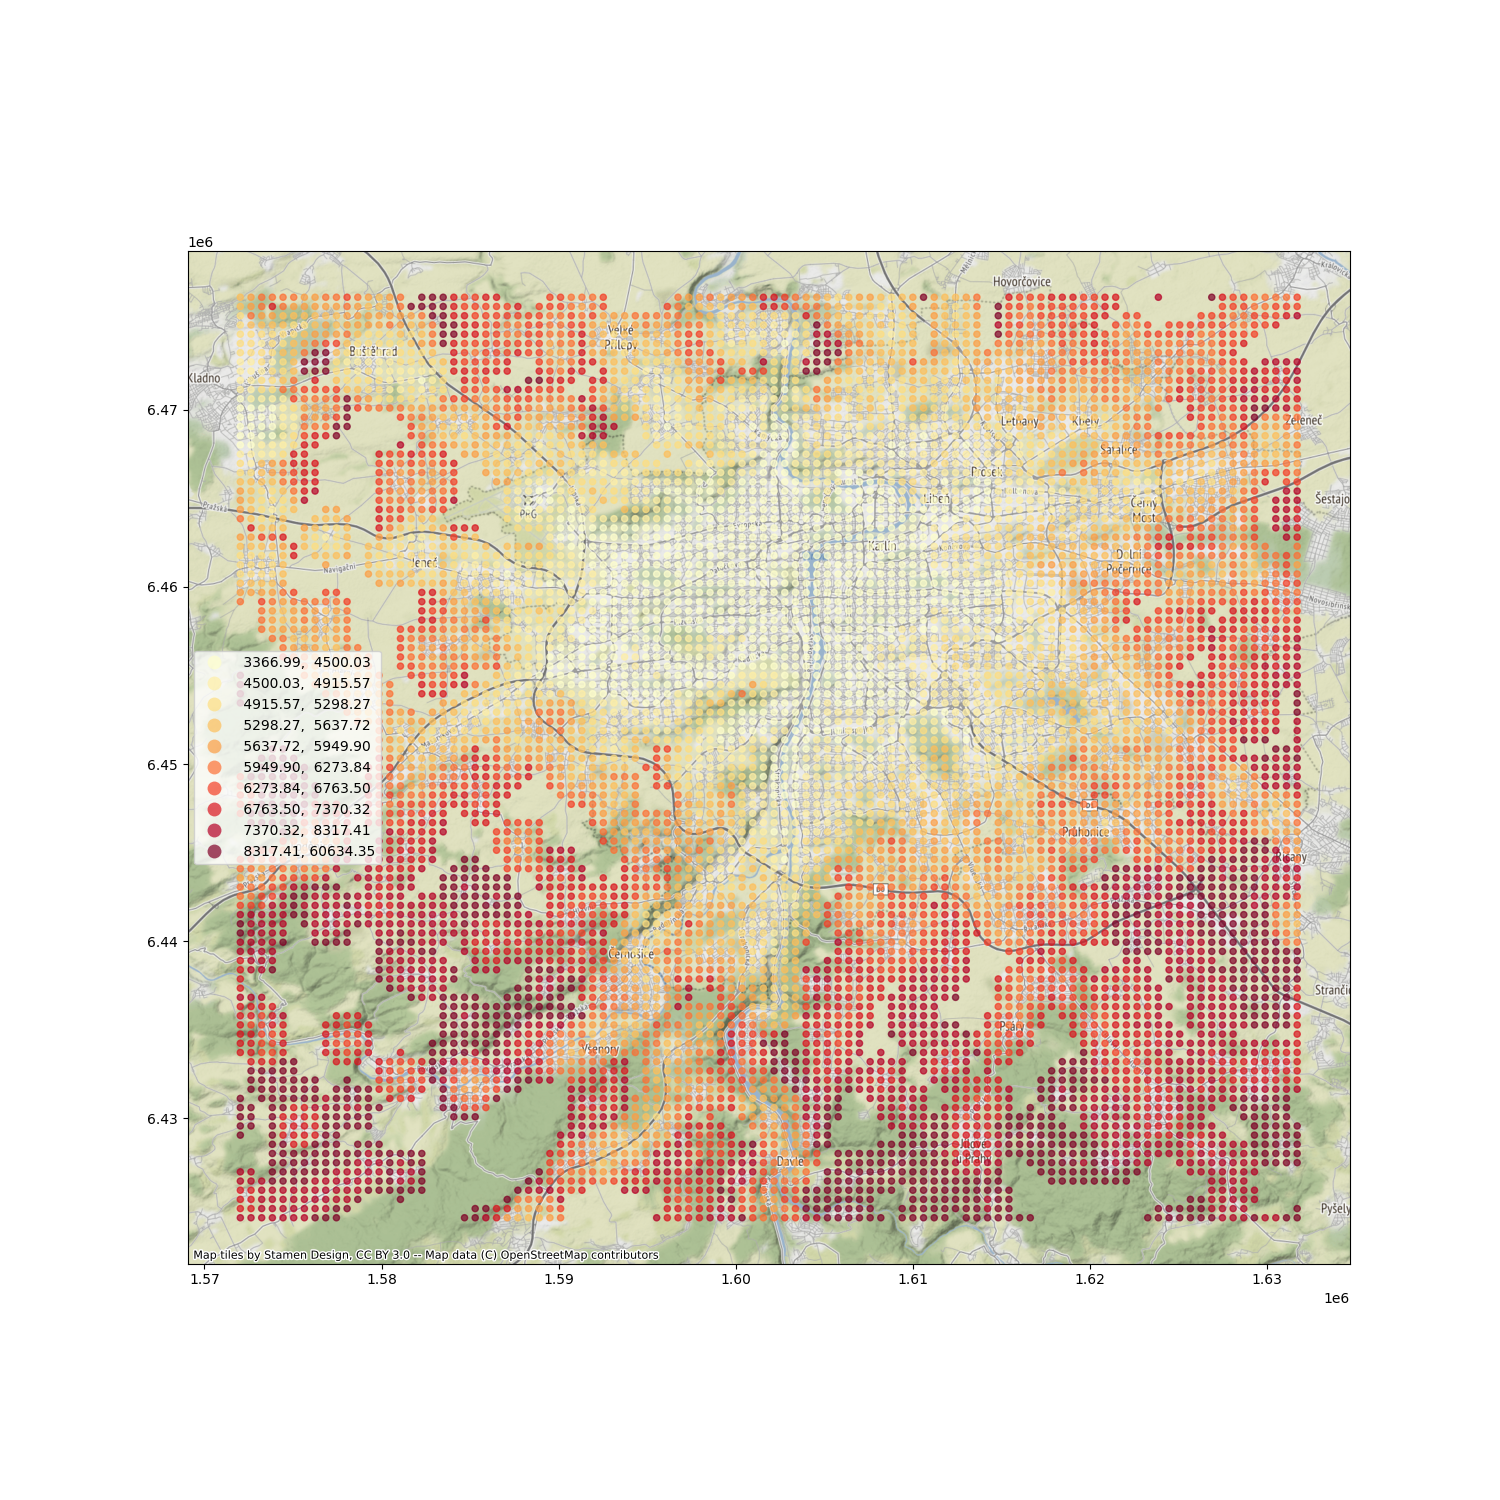
\includegraphics[width=\textwidth]{../img/staticPlaceVisualization.png}
    \caption{Vizualizace dostupnosti v~rastru 100~x~100 z~Malostranského náměstí, Kladna a~Příbrami. Hodnoty v~legendě vyjadřují dostupnost v~sekundách.}
    \label{fig:gtfs-mostAccessiblePlace}
\end{figure}


\section{Interaktivní vizualizace}\label{Interaktivni-vizualizace}

Dostupnost můžeme vizualizovat v~interaktivní mapě. Tím umožníme uživatelům nejen zobrazovat výsledky na mapě, ale také pohybovat se po mapě a~zjišťovat tak dostupnost na konkrétních místech.

Vizualizaci zpřístupníme uživatelům skrze webovou aplikaci. Z~toho důvodu jsme pro implementaci vizualizace zvolili jazyk JavaScript.

\subsubsection{Výběr knihovny}

Při implementaci této vizualizace budeme chtít využít existující knihovnu, abychom si ušetřili práci. Knihoven pro práci s~interaktivní mapou existuje mnoho. Zvážíme následující možnosti.

\begin{enumerate}
    \item Google map API. Google sice umožňuje využívat API po dobu prvního půl roku zdarma, obecně se ale jedná o~placenou službu.
    \item Mapquest. Placená knihovna, prvních 15 000 transakcí by mělo být zdarma.
    \item OpenLayers. Open-source knihovna, zcela zdarma.
\end{enumerate}

Preferovanou knihovnou je OpenLayers, neboť je jako jediná zdarma. Nenutí nás tedy vynucovat poplatky na uživatelích aplikace. Navíc nevynucuje žádné komerční závislosti pro případné další vývojáře naší aplikace.

\subsubsection{OpenLayers}

Knihovna OpenLayers používá jako výchozí projekci WGS84 (World Geodetic System). Stejná projekce je použita i~pro geografická data popsaná ve formátu GTFS. To nám ušetří práci s~případnými konverzemi projekcí.

Umožňuje kreslení na podklad map z~OSM (OpenStreetMap). Jedná se o~volně dostupné mapy, pro nás tedy ideální volba.

Pracuje s~vizualizačními vrstvami, není tedy problém přidat vrstvu obsahující vizualizované body a~vrstvu obsahující uživatelem zadaná vstupní místa pro výpočet dostupnosti.

Umí pracovat s~WebGL (Web Graphics Library), které umožňuje rychlejší vykreslování velkého množství bodů.

\subsubsection{Výsledná vizualizace}

Následující obrázky zobrazují interaktivní vizualizaci dostupností na zastávkách, viz obrázek~\ref{fig:ol-vizualizace-zastavek} a~vizualizaci dostupností na bodech v~rastru, viz obrázek~\ref{fig:ol-vizualizace-mist}.

\begin{figure}[ht]
    \centering
    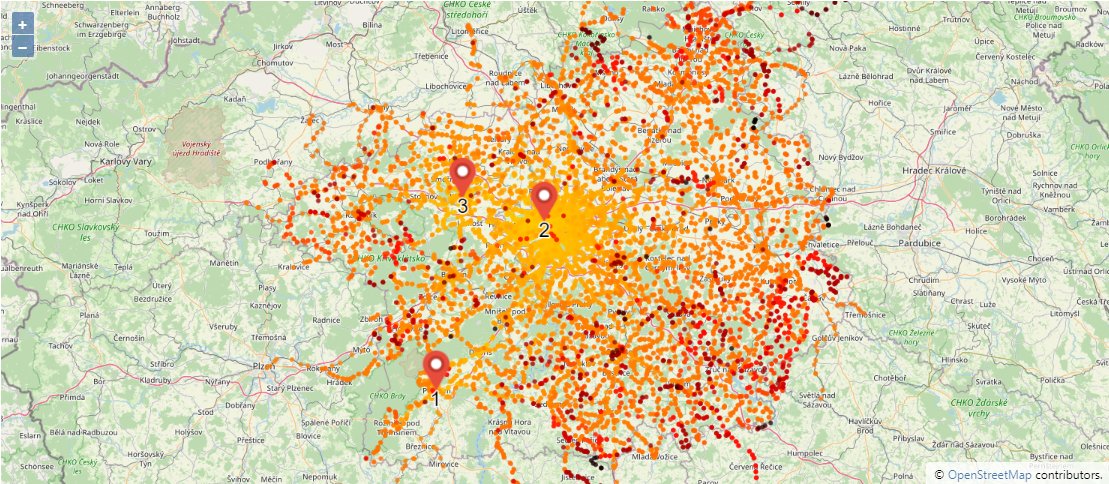
\includegraphics[width=\textwidth]{../img/interactiveStopVisualization.png}
    \caption{Interaktivní vizualizace dostupnosti na zastávkách z~Malostranského náměstí, Kladna a~Příbrami.}
    \label{fig:ol-vizualizace-zastavek}
\end{figure}

\begin{figure}[ht]
    \centering
    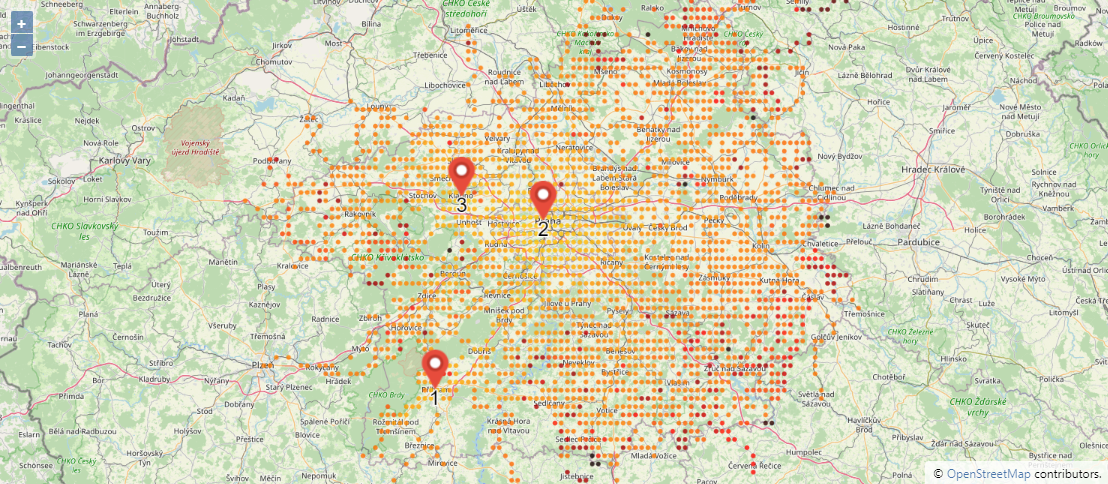
\includegraphics[width=\textwidth]{../img/interactivePlaceVisualization.png}
    \caption{Interaktivní vizualizace dostupnosti v~rastru 100~x~100 z~Malostranského náměstí, Kladna a~Příbrami.}
    \label{fig:ol-vizualizace-mist}
\end{figure}

\section{Možné vylepšení}

Spíše než vizualizace bodů by pro uživatele mohla být zajímavější možnost vizualizace pomocí jednolitého barevného filtru, který by překrýval mapu.

Základem takového filtru by byla dostupnost v~bodech. Dostupnost na místech mezi body bychom mohli interpolovat pomocí dostupností na okolních bodech.
